
% ----------------------------------------------------------
% CAPÍTULO 04 - RESULTADOS
% ----------------------------------------------------------

\chapter{Simulação e Resultados} \label{cha:resultados}

Este capítulo contextualiza e descreve os choques exógenos planejados para serem aplicados no modelo de equilíbrio geral. Em seguida, são apresentados os resultados do modelo, analisando os efeitos macroeconômicos quanto setoriais, permitindo conseguintemente mensurar a natureza do impacto sobre o modelo e quais foram os grupos beneficiados e prejudicados por ele.

A simulação proposta tem o objetivo de avaliar o efeito de curto prazo do comércio internacional sobre a desigualdade de renda e pobreza no Brasil. Nela, impõe-se uma redução tarifária de 25\% para todos os setores da economia. A ideia é investigar como uma mudança significante afetaria a produção, salários e emprego, além das variáveis setoriais.


\section{Resultados macroeconômicos} \label{sec:resultados_macro}

\begin{table}[h]
	\centering
	\begin{threeparttable}
		\caption{resultados macroeconômicos de curto-prazo} \label{tab:macro}
		\begin{tabular}{lcc}
			\toprule
			\multicolumn{1}{c}{\textbf{descrição}} & \textbf{variável} & \textbf{valor} \\ \hline
			Volume de exportações                   & $x4tot$          & 6,13 \\
			Volume de importações (CIF)             & $x0cif\_c$       & 11,47 \\
			PIB real (ótica da despesa)             & $x0gdpexp$       & \textcolor{red}{0,78} \\
			Estoque de capital agregado             & $x1cap\_i$       & 0,000 \\
			Emprego agregado                        & $employ\_i$      & \textcolor{red}{1,38} \\
			Índice de Preço de Absorção             & $p0gne$          & \textcolor{red}{1,78} \\
			Índice de preços do PIB                 & $p0gdpexp$       & \textcolor{red}{2,53} \\
			IPC                                     & $p3tot$          & \textcolor{red}{0,23} \\
			Índice de preços das exportações        & $p4tot$          & \textcolor{red}{5,52} \\
			Desvalorização real                     & $p0realdev$      & 2,59 \\
			Salário médio nominal                   & $p1lab\_io$      & \textcolor{red}{0,23} \\
			Part. da Balança comercial sobre o PIB  & $ContBOT$        & \textcolor{red}{0,78} \\
			Termos de troca                         & $p0toft$         & \textcolor{red}{5,52} \\
			Variação em nível da receita tarifária  & $delV0tar\_c$    & \textcolor{red}{230.448,38} \\
			\bottomrule
		\end{tabular}
		\begin{tablenotes}
			\small
			\item Fonte: elaboração própria (2023) com base nos dados do ORANIG-BR.
			\item \textit{Nota}: células em vermelho representam variações negativas.
		\end{tablenotes}
		\end{threeparttable}
	\end{table}

A partir da Tabela \ref{tab:macro}, percebe-se que o corte tarifário prejudicou o desempenho da economia no curto-prazo, gerando perda de competitividade internacional. O volume importado aumentou consideravelmente (11,47\%), reflexo do barateamento do produto estrangeiro frente ao doméstico. Esse desbalanço provocou uma queda de 5,52\% dos termos de troca que, somados a uma perda considerável da receita tarifária, afastou qualquer possibilidade de um saldo positivo no cenário macroeconômico. Desse modo, experimentou-se uma redução nos postos de emprego (-1,38\%), nos salários (-0,23\%) e no PIB (-0,78\%).
 
É válido ressaltar que a corrente de comércio influenciou tão significativamente no comportamento das variáveis macroeconômicas por conta do fechamento adotado. Todas as variáveis do PIB real estão exógenas - com a exceção da balança comercial. Desse modo, bastou a variação das importações ser maior que o das exportações para resultar numa piora dos indicadores econômicos.

Ainda assim, o resultado encontrado é convergente com a literatura econômica, uma vez que um país em desenvolvimento mais integrado ao comércio internacional também pode estar mais vulnerável a choques externos. como mudanças abruptas nos termos de troca \cite{bannisterthugge01, winters02}.


\section{Resultados setoriais} \label{sec:resultados_setoriais}

O Gráfico \ref{fig:fandecomp} mostra o comportamento da variável $fandecomp$ - que significa a decomposição da demanda dos 124 insumos produzidos internamente. Nele, é possível perceber que os produtos relacionados a manufatura foram os mais afetados pelo corte tarifário. Os insumos FioFibraTex e Tecidos obtiveram as maiores reduções na demanda pela produção, puxados pelo aumento na preferência dos insumos importados e redução na própria demanda do mercado interno.

Por outro lado, o insumo AeroEmbOut aumentou em 5,3\% sua produção - majoritariamente para atender o mercado externo. Esse fenômeno está ligado à redução dos custos de produção do setor, que utiliza uma parcela significativa de insumos importados para produzir. Desse modo, o corte tarifário funcionou, indiretamente, como um choque de produtividade para o setor, aumento sua produção direcionada ao mercado internacional.

\begin{figure}[h]
	\centering
	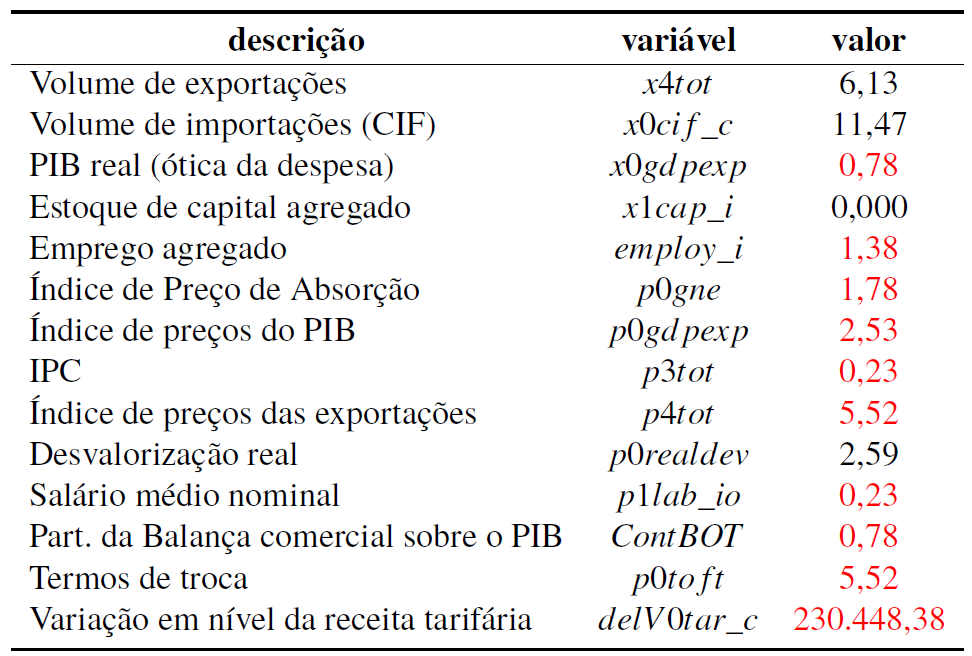
\includegraphics[width=\linewidth]{Imagens/006.png}
	\caption{resultados da variável \textit{fan decomposition}}
	\label{fig:fandecomp}
	\footnotesize
	Fonte: elaboração própria (2023) com base nos dados do ORANIG-BR.
\end{figure}

A mesma lógica pode ser encontradas ao analisar a produção e investimento setoriais. Percebe-se que o corte tarifário fomentou a produção dos setores cuja estrutura de custos era mais permeada por insumos importados. Os setores de fabricação de equipamentos de transporte e extração mineral foram os maiores beneficiados. Por outro lado, os setores mais voltados para o mercado interno, com pouca aderência ao comércio internacional, foram os maiores prejudicados, podendo citar o setor de têxteis (-7,75\%) e alojamento (-7,17\%). 

\begin{figure}[h]
	\centering
	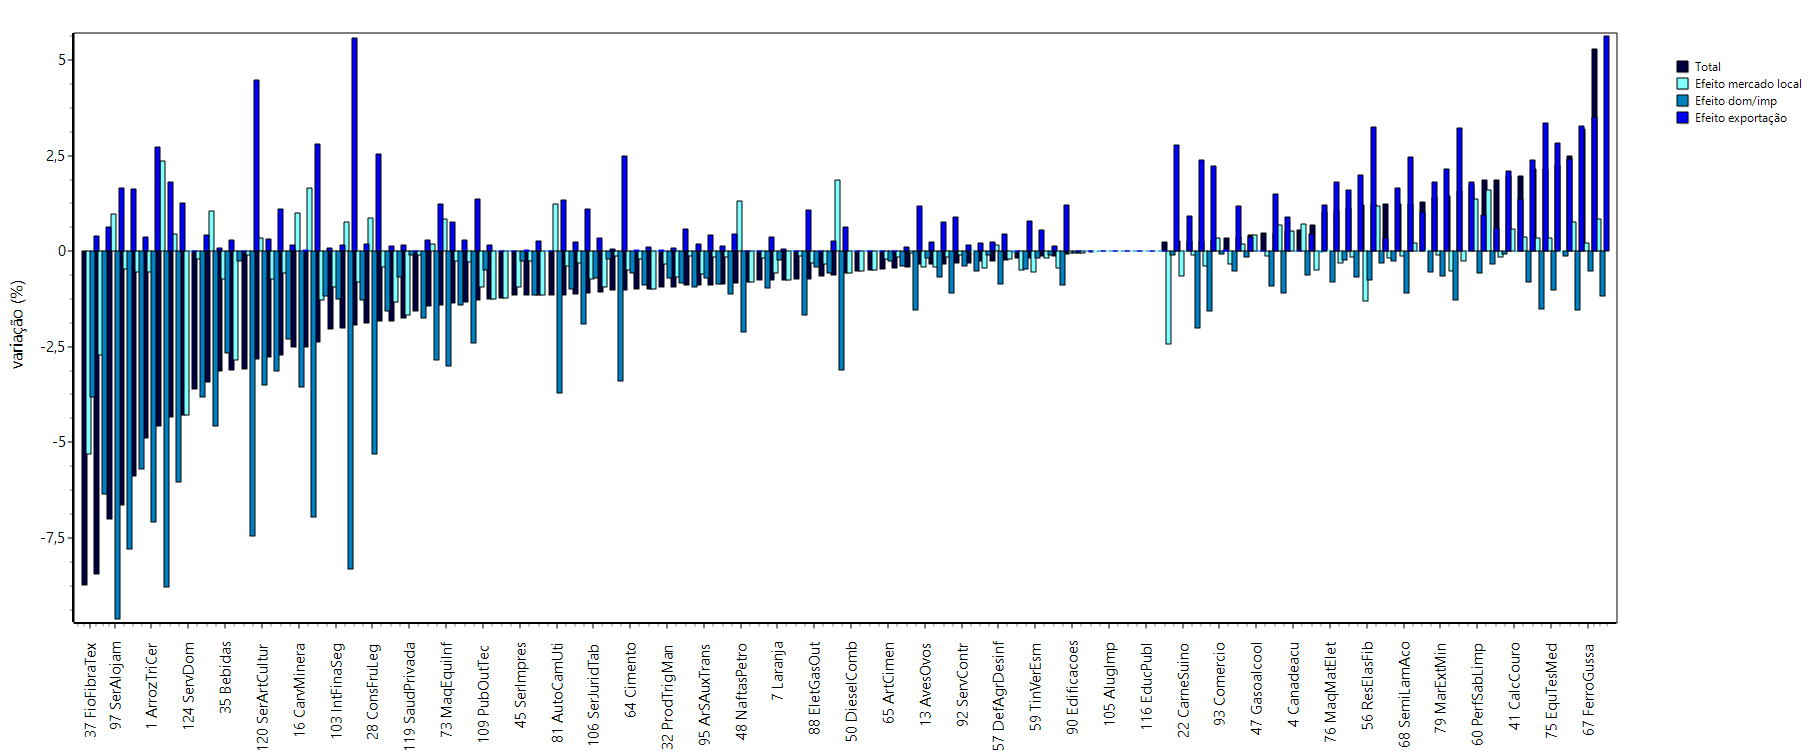
\includegraphics[width=\linewidth]{Imagens/007.png}
	\caption{produção e investimento setorial}
	\label{fig:x1x2}
	\footnotesize
	Fonte: elaboração própria (2023) com base nos dados do ORANIG-BR.
\end{figure}

Desse modo, pode-se afirmar que o corte tarifário reduziu o preço dos insumos importados, tornando-os mais atrativos comparativamente aos domésticos. Essa redução se apresentou, para os setores com maior adesão ao comércio internacional, como um choque positivo de produtividade, elevando seu grau de investimento e de produtividade. Entretanto, esse impacto setorial não foi o suficiente para gerar ganho líquido. A deterioração dos termos de troca, somado a uma relevante perda de receita tarifária, fizeram com que os indicadores macroeconômicos sofressem uma piora, havendo queda do PIB, emprego e salários.


